% !TeX spellcheck = ru_RU
% !TEX root = vkr.tex

\section{Общая архитектура проекта}
\label{sec:big-arch}

Проект \Lamagraph{} ставит перед собой цель изучить возможности по созданию специализированных ускорителей на основе \INs{}.

К проекту выдвинуты следующие требования.
\begin{itemize}
    \item Возможность параметризовать компилятор и вычислительное ядро типами агентов сети и правилами их редукции.
    \item Возможность сбора статистики такой, как размер сети, количество редукций, время исполнения и другой.
    \item Возможность постановки сравнительных экспериментов.
    \item Использование единого стека технологий~--- гомогенность.
    \item Получение полнофункционального прототипа, содержащего все компоненты, важнее, чем детальная проработка какого-то отдельного компонента.
    \item Расширяемость и модифицируемость.
          Должна быть возможность вносить изменения в любые компоненты.
\end{itemize}


Крупномасштабная архитектура проекта изображена на рисунке~\ref{fig:lamagraph-big} и состоит из трёх крупных блоков.
\begin{description}
    \item[Compiler] Транслятор ML-подобного языка программирования.
          Содержит в себе интерпретатор и генерирует промежуточное представление, пригодное к дальнейшей трансляции в \INs{}.
    \item[Hardware] Генератор описания аппаратуры для ПЛИС, параметризуемый базисом агентов сети.
    \item[Middle] Транслятор из промежуточного представления в байт-код, пригодный для исполнения на процессоре, сгенерированном в блоке Hardware.
\end{description}


Проект является командным.
Блоки Compiler и Hardware достаточно независимы друг от друга.
Блок Middle объединяет два других, поэтому его разработка должна быть скоординирована.
В данной работе речь пойдёт о блоке Compiler.

\begin{figure}
    \begin{center}
        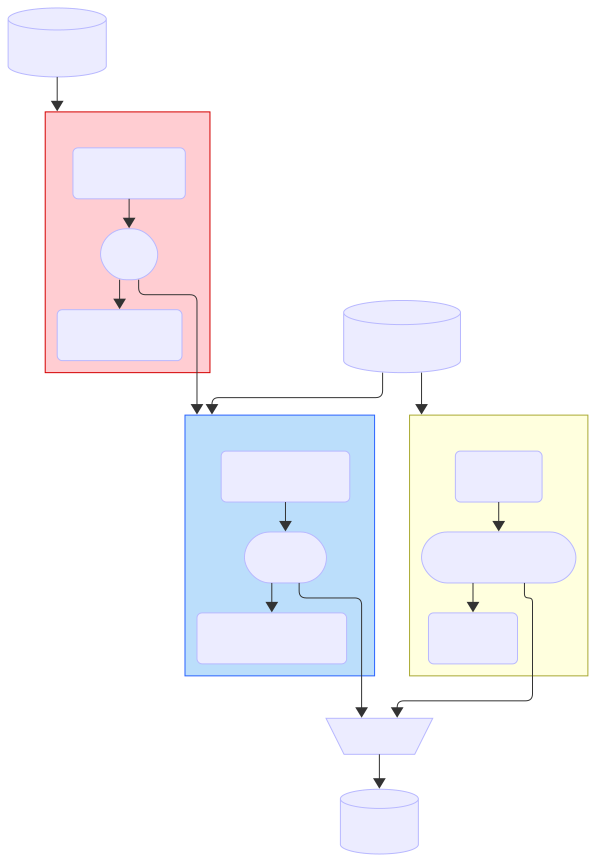
\includegraphics[width=0.6\linewidth]{lamagraph-big}
    \end{center}
    \caption{Общая архитектура проекта \Lamagraph{}.}
    \label{fig:lamagraph-big}
\end{figure}
